%begin-include

%In this chapter we present experiments of model selection of cell
% signaling pathways. We divide this chapter in two sections; the first
% section presents experiments to compare two model selection software: 
% ABC-SMC and SigNetMS, both of them presented on
% chapter~\ref{chap:model_selection_methods}. We end the first section
% presenting which software had best fit for our experiments. The
% following section presents experiments of model selection as a feature
% selection problem. We will analyze algorithm trace and what is the
% surface induced by the cost function over the search space.

\section{Choosing a Software for Model Selection}
% To choose a software for model selection we did the same experiment as
% girolami
%
% A simple instance of the model selection problem
% -> the correct model is...
% -> then we create other three models
%   - a simplification
%   - an overly complex model
%   - and an incorrect model
% -> the expected result for this experiment is that the correct model
%  has a higher (possibly be the first), and that the incorrect model
%  should be considered the worst. It is also important to see how the
%  software compares models with similar dynamics and with different
%  levels of complexity.
%  
% Results produced by SigNetMS and ABC-SysBio
% -> we proceeded to run both softwares 
% -> compare the ranking of both software
% -> show how the curve fits on both software
% -> show that there is some parameter value convergence on SigNetMS

To choose between SigNetMS and ABC-SysBio, we performed a model
selection experiment. This experiment, originally performed on the work
of Vyshemirsky and Girolami~\cite{Vyshemirsky2007}, consists in creating
artificial experimental data from a model of cell signaling pathway, and 
then selecting between four different models, including the correct one.
Using SigNetMS and ABC-SysBio we should be able to create a ranking of
the four models, in which we expect to see as the best, the model we
used to create the experimental data. More than that, we should analyze
the produced results to check if simpler models are preferred over
complex models; we should also check if the simulations produced by the
models, with the estimated sample of the posterior distribution of
parameters, approximates experimental data.

\subsection{A simple instance of the model selection problem}
We start our model selection problem with the correct model, which is 
a signalling pathway composed by five reactions and five chemical 
species. Figure~\ref{fig:experiments:girolami1} shows a diagram with
this model. This model represents a common motif, and it has as the 
input signal the chemical species "S", and as the output the chemical 
species "Rpp"; the experimental measurement used is the concentration of 
the output chemical species, which we donote as [Rpp].

\begin{figure}
\begin{center}
    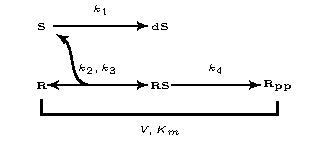
\includegraphics[width=.75\textwidth]{experiments/diagrams/bioinformatics_model1.pdf}
    \caption{Caption to the model}
    \label{fig:experiments:girolami}
    \end{center}

\end{figure}

In this experiment, for the sake of simplicity, we neglect the units of 
reaction rates constants and initial concentrations. The initial 
concentrations used are:  S $= 1$, R $= 1$, dS $= 0$, RS $= 0$, 
R$_{pp} = 0$. To create the experimental data, the reaction rate 
constants we used have the values: 
$k_1 = 0.07$, $k_2 = 0.6$, $k_3 = 0.05$, $k_4 = 0.3$, $V = 0.017$, and
$K_m = 0.3$. It is important to remember that we discard reaction rate
constant values during model selection; initial concentrations, however,
are still provided during this phase.

% insert simulated data here

\section{Model Selection as a Feature Selection Problem}
